\documentclass{standalone}
\usepackage{tikz}
\usetikzlibrary{patterns, positioning}

\begin{document}
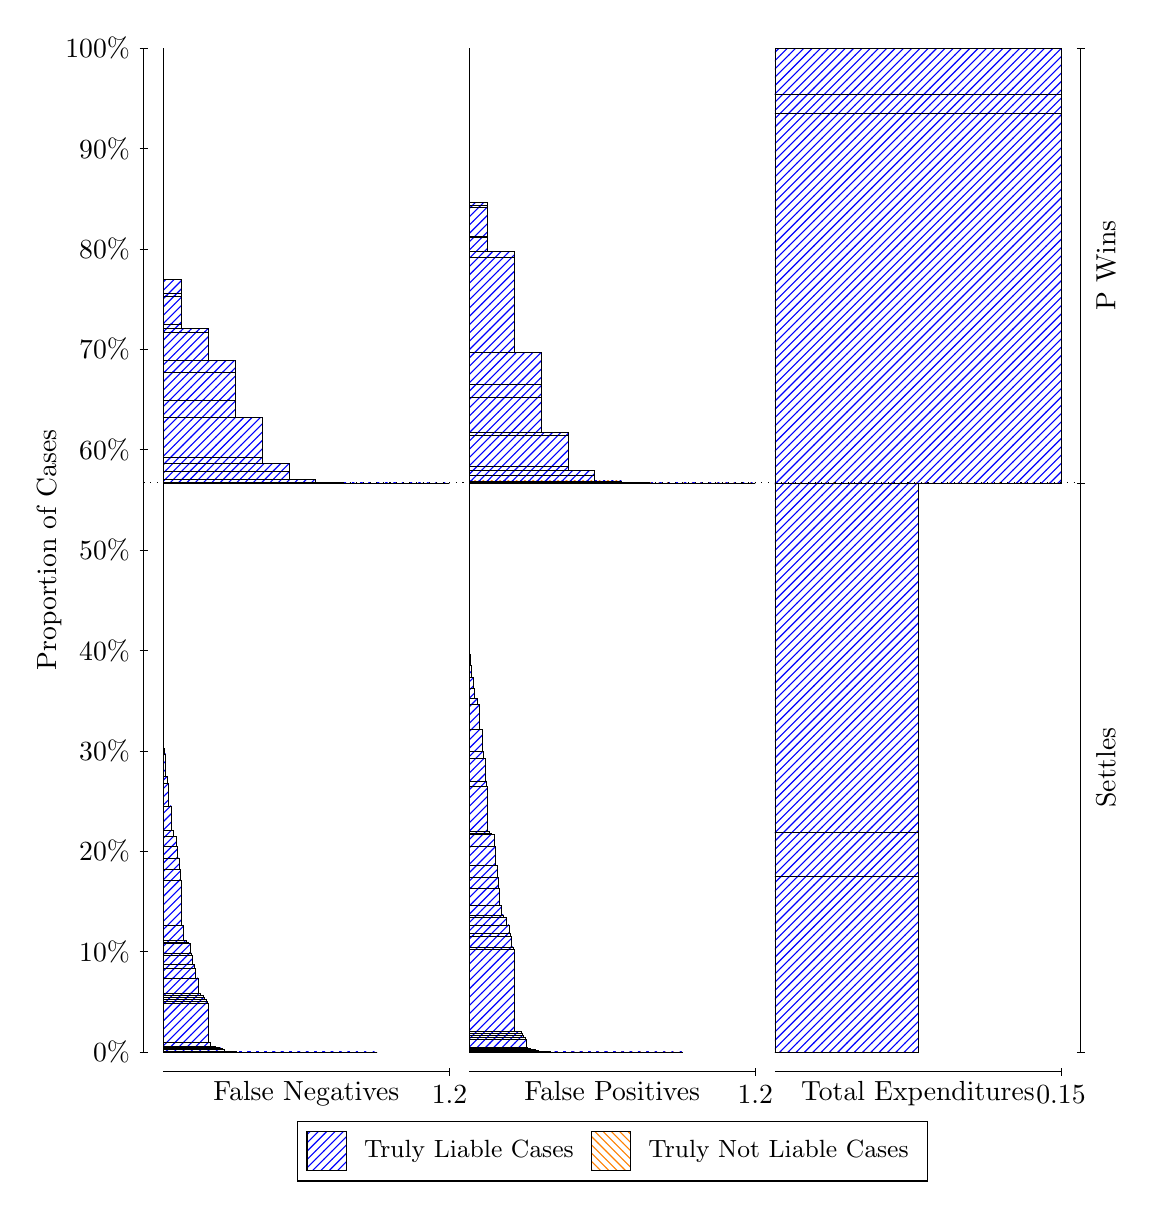
\begin{tikzpicture}
\draw[black, very thin] (1.5,1.75) -- (1.5,14.5);
\node[rotate=90, anchor=center] at (0.3, 8.125) {Proportion of Cases};
\draw[black, very thin] (1.45,1.75) -- (1.55,1.75);
\node[anchor=east] at (1.45, 1.75) {0\%};
\draw[black, very thin] (1.45,3.025) -- (1.55,3.025);
\node[anchor=east] at (1.45, 3.025) {10\%};
\draw[black, very thin] (1.45,4.3) -- (1.55,4.3);
\node[anchor=east] at (1.45, 4.3) {20\%};
\draw[black, very thin] (1.45,5.575) -- (1.55,5.575);
\node[anchor=east] at (1.45, 5.575) {30\%};
\draw[black, very thin] (1.45,6.85) -- (1.55,6.85);
\node[anchor=east] at (1.45, 6.85) {40\%};
\draw[black, very thin] (1.45,8.125) -- (1.55,8.125);
\node[anchor=east] at (1.45, 8.125) {50\%};
\draw[black, very thin] (1.45,9.4) -- (1.55,9.4);
\node[anchor=east] at (1.45, 9.4) {60\%};
\draw[black, very thin] (1.45,10.675) -- (1.55,10.675);
\node[anchor=east] at (1.45, 10.675) {70\%};
\draw[black, very thin] (1.45,11.95) -- (1.55,11.95);
\node[anchor=east] at (1.45, 11.95) {80\%};
\draw[black, very thin] (1.45,13.225) -- (1.55,13.225);
\node[anchor=east] at (1.45, 13.225) {90\%};
\draw[black, very thin] (1.45,14.5) -- (1.55,14.5);
\node[anchor=east] at (1.45, 14.5) {100\%};

\draw[black, very thin] (13.4,1.75) -- (13.4,14.5);
\draw[black, very thin] (13.35,1.75) -- (13.45,1.75);
\node[anchor=west] at (13.35, 1.75) {};
\draw[black, very thin] (13.35,8.9775) -- (13.45,8.9775);
\node[anchor=west] at (13.35, 8.9775) {};
\draw[black, very thin] (13.35,14.5) -- (13.45,14.5);
\node[anchor=west] at (13.35, 14.5) {};

\draw[black, very thin, pattern color=blue, pattern=north east lines] (1.75,1.75) rectangle (4.4654,1.75);
\draw[black, very thin, pattern color=blue, pattern=north east lines] (1.75,1.75) rectangle (4.3125,1.75);
\draw[black, very thin, pattern color=blue, pattern=north east lines] (1.75,1.75) rectangle (4.1595,1.75);
\draw[black, very thin, pattern color=blue, pattern=north east lines] (1.75,1.75) rectangle (4.1255,1.75);
\draw[black, very thin, pattern color=blue, pattern=north east lines] (1.75,1.75) rectangle (4.0065,1.75);
\draw[black, very thin, pattern color=blue, pattern=north east lines] (1.75,1.75) rectangle (3.9725,1.75);
\draw[black, very thin, pattern color=blue, pattern=north east lines] (1.75,1.75) rectangle (3.8535,1.75);
\draw[black, very thin, pattern color=blue, pattern=north east lines] (1.75,1.75) rectangle (3.8195,1.75);
\draw[black, very thin, pattern color=blue, pattern=north east lines] (1.75,1.75) rectangle (3.7855,1.75);
\draw[black, very thin, pattern color=blue, pattern=north east lines] (1.75,1.75) rectangle (3.7005,1.75);
\draw[black, very thin, pattern color=blue, pattern=north east lines] (1.75,1.75) rectangle (3.6665,1.75);
\draw[black, very thin, pattern color=blue, pattern=north east lines] (1.75,1.75) rectangle (3.6325,1.75);
\draw[black, very thin, pattern color=blue, pattern=north east lines] (1.75,1.75) rectangle (3.5475,1.75);
\draw[black, very thin, pattern color=blue, pattern=north east lines] (1.75,1.75) rectangle (3.5135,1.75);
\draw[black, very thin, pattern color=blue, pattern=north east lines] (1.75,1.75) rectangle (3.4796,1.75);
\draw[black, very thin, pattern color=blue, pattern=north east lines] (1.75,1.75) rectangle (3.4456,1.75);
\draw[black, very thin, pattern color=blue, pattern=north east lines] (1.75,1.75) rectangle (3.3946,1.75);
\draw[black, very thin, pattern color=blue, pattern=north east lines] (1.75,1.75) rectangle (3.3606,1.75);
\draw[black, very thin, pattern color=blue, pattern=north east lines] (1.75,1.75) rectangle (3.3266,1.75);
\draw[black, very thin, pattern color=blue, pattern=north east lines] (1.75,1.75) rectangle (3.2926,1.75);
\draw[black, very thin, pattern color=blue, pattern=north east lines] (1.75,1.75) rectangle (3.2416,1.75);
\draw[black, very thin, pattern color=blue, pattern=north east lines] (1.75,1.75) rectangle (3.2076,1.75);
\draw[black, very thin, pattern color=blue, pattern=north east lines] (1.75,1.75) rectangle (3.1736,1.75);
\draw[black, very thin, pattern color=blue, pattern=north east lines] (1.75,1.75) rectangle (3.1396,1.75);
\draw[black, very thin, pattern color=blue, pattern=north east lines] (1.75,1.75) rectangle (3.1056,1.75);
\draw[black, very thin, pattern color=blue, pattern=north east lines] (1.75,1.75) rectangle (3.0886,1.75);
\draw[black, very thin, pattern color=blue, pattern=north east lines] (1.75,1.75) rectangle (3.0546,1.75);
\draw[black, very thin, pattern color=blue, pattern=north east lines] (1.75,1.75) rectangle (3.0206,1.75);
\draw[black, very thin, pattern color=blue, pattern=north east lines] (1.75,1.75) rectangle (2.9866,1.75);
\draw[black, very thin, pattern color=blue, pattern=north east lines] (1.75,1.75) rectangle (2.9526,1.75);
\draw[black, very thin, pattern color=blue, pattern=north east lines] (1.75,1.75) rectangle (2.9356,1.75);
\draw[black, very thin, pattern color=blue, pattern=north east lines] (1.75,1.75) rectangle (2.9016,1.7501);
\draw[black, very thin, pattern color=blue, pattern=north east lines] (1.75,1.7501) rectangle (2.8676,1.7506);
\draw[black, very thin, pattern color=blue, pattern=north east lines] (1.75,1.7506) rectangle (2.8336,1.7507);
\draw[black, very thin, pattern color=blue, pattern=north east lines] (1.75,1.7507) rectangle (2.7996,1.7508);
\draw[black, very thin, pattern color=blue, pattern=north east lines] (1.75,1.7508) rectangle (2.7826,1.7508);
\draw[black, very thin, pattern color=blue, pattern=north east lines] (1.75,1.7508) rectangle (2.7656,1.7509);
\draw[black, very thin, pattern color=blue, pattern=north east lines] (1.75,1.7509) rectangle (2.7486,1.7509);
\draw[black, very thin, pattern color=blue, pattern=north east lines] (1.75,1.7509) rectangle (2.7146,1.751);
\draw[black, very thin, pattern color=blue, pattern=north east lines] (1.75,1.751) rectangle (2.6806,1.7533);
\draw[black, very thin, pattern color=blue, pattern=north east lines] (1.75,1.7533) rectangle (2.6466,1.754);
\draw[black, very thin, pattern color=blue, pattern=north east lines] (1.75,1.754) rectangle (2.6296,1.7553);
\draw[black, very thin, pattern color=blue, pattern=north east lines] (1.75,1.7553) rectangle (2.6127,1.7558);
\draw[black, very thin, pattern color=blue, pattern=north east lines] (1.75,1.7558) rectangle (2.5957,1.7565);
\draw[black, very thin, pattern color=blue, pattern=north east lines] (1.75,1.7565) rectangle (2.5617,1.7585);
\draw[black, very thin, pattern color=blue, pattern=north east lines] (1.75,1.7585) rectangle (2.5277,1.782);
\draw[black, very thin, pattern color=blue, pattern=north east lines] (1.75,1.782) rectangle (2.4937,1.7914);
\draw[black, very thin, pattern color=blue, pattern=north east lines] (1.75,1.7914) rectangle (2.4767,1.8014);
\draw[black, very thin, pattern color=blue, pattern=north east lines] (1.75,1.8014) rectangle (2.4597,1.808);
\draw[black, very thin, pattern color=blue, pattern=north east lines] (1.75,1.808) rectangle (2.4427,1.8101);
\draw[black, very thin, pattern color=blue, pattern=north east lines] (1.75,1.8101) rectangle (2.4257,1.8158);
\draw[black, very thin, pattern color=blue, pattern=north east lines] (1.75,1.8158) rectangle (2.4087,1.8188);
\draw[black, very thin, pattern color=blue, pattern=north east lines] (1.75,1.8188) rectangle (2.3747,1.8218);
\draw[black, very thin, pattern color=blue, pattern=north east lines] (1.75,1.8218) rectangle (2.3407,1.8701);
\draw[black, very thin, pattern color=blue, pattern=north east lines] (1.75,1.8701) rectangle (2.3237,2.3738);
\draw[black, very thin, pattern color=blue, pattern=north east lines] (1.75,2.3738) rectangle (2.3067,2.3974);
\draw[black, very thin, pattern color=blue, pattern=north east lines] (1.75,2.3974) rectangle (2.2897,2.4243);
\draw[black, very thin, pattern color=blue, pattern=north east lines] (1.75,2.4243) rectangle (2.2727,2.4448);
\draw[black, very thin, pattern color=blue, pattern=north east lines] (1.75,2.4448) rectangle (2.2557,2.4661);
\draw[black, very thin, pattern color=blue, pattern=north east lines] (1.75,2.4661) rectangle (2.2217,2.4975);
\draw[black, very thin, pattern color=blue, pattern=north east lines] (1.75,2.4975) rectangle (2.1877,2.6919);
\draw[black, very thin, pattern color=blue, pattern=north east lines] (1.75,2.6919) rectangle (2.1537,2.8147);
\draw[black, very thin, pattern color=blue, pattern=north east lines] (1.75,2.8147) rectangle (2.1367,2.8701);
\draw[black, very thin, pattern color=blue, pattern=north east lines] (1.75,2.8701) rectangle (2.1197,2.9771);
\draw[black, very thin, pattern color=blue, pattern=north east lines] (1.75,2.9771) rectangle (2.1027,3.0071);
\draw[black, very thin, pattern color=blue, pattern=north east lines] (1.75,3.0071) rectangle (2.0857,3.1251);
\draw[black, very thin, pattern color=blue, pattern=north east lines] (1.75,3.1251) rectangle (2.0687,3.1443);
\draw[black, very thin, pattern color=blue, pattern=north east lines] (1.75,3.1443) rectangle (2.0347,3.1635);
\draw[black, very thin, pattern color=blue, pattern=north east lines] (1.75,3.1635) rectangle (2.0007,3.3565);
\draw[black, very thin, pattern color=blue, pattern=north east lines] (1.75,3.3565) rectangle (1.9837,3.9278);
\draw[black, very thin, pattern color=blue, pattern=north east lines] (1.75,3.9278) rectangle (1.9667,4.0715);
\draw[black, very thin, pattern color=blue, pattern=north east lines] (1.75,4.0715) rectangle (1.9497,4.2147);
\draw[black, very thin, pattern color=blue, pattern=north east lines] (1.75,4.2147) rectangle (1.9327,4.3641);
\draw[black, very thin, pattern color=blue, pattern=north east lines] (1.75,4.3641) rectangle (1.9157,4.4873);
\draw[black, very thin, pattern color=blue, pattern=north east lines] (1.75,4.4873) rectangle (1.8817,4.5665);
\draw[black, very thin, pattern color=blue, pattern=north east lines] (1.75,4.5665) rectangle (1.8477,4.8762);
\draw[black, very thin, pattern color=blue, pattern=north east lines] (1.75,4.8762) rectangle (1.8137,5.1565);
\draw[black, very thin, pattern color=blue, pattern=north east lines] (1.75,5.1565) rectangle (1.7967,5.2509);
\draw[black, very thin, pattern color=blue, pattern=north east lines] (1.75,5.2509) rectangle (1.7797,5.5345);
\draw[black, very thin, pattern color=blue, pattern=north east lines] (1.75,5.5345) rectangle (1.7627,5.6091);
\draw[black, very thin, pattern color=orange, pattern=north west lines] (1.75,5.6091) rectangle (1.75,5.6091);
\draw[black, very thin, pattern color=blue, pattern=north east lines] (1.75,5.6091) rectangle (1.75,8.9775);
\draw[black, very thin, pattern color=blue, pattern=north east lines] (1.75,8.9775) rectangle (5.3833,8.9775);
\draw[black, very thin, pattern color=blue, pattern=north east lines] (1.75,8.9775) rectangle (5.0434,8.9775);
\draw[black, very thin, pattern color=blue, pattern=north east lines] (1.75,8.9775) rectangle (4.7034,8.9775);
\draw[black, very thin, pattern color=blue, pattern=north east lines] (1.75,8.9775) rectangle (4.7034,8.9775);
\draw[black, very thin, pattern color=blue, pattern=north east lines] (1.75,8.9775) rectangle (4.3635,8.9777);
\draw[black, very thin, pattern color=blue, pattern=north east lines] (1.75,8.9777) rectangle (4.3635,8.9779);
\draw[black, very thin, pattern color=blue, pattern=north east lines] (1.75,8.9779) rectangle (4.0235,8.9831);
\draw[black, very thin, pattern color=blue, pattern=north east lines] (1.75,8.9831) rectangle (4.015,8.9831);
\draw[black, very thin, pattern color=blue, pattern=north east lines] (1.75,8.9831) rectangle (3.6835,9.0237);
\draw[black, very thin, pattern color=blue, pattern=north east lines] (1.75,9.0237) rectangle (3.675,9.0237);
\draw[black, very thin, pattern color=blue, pattern=north east lines] (1.75,9.0237) rectangle (3.3436,9.126);
\draw[black, very thin, pattern color=blue, pattern=north east lines] (1.75,9.126) rectangle (3.3436,9.2229);
\draw[black, very thin, pattern color=blue, pattern=north east lines] (1.75,9.2229) rectangle (3.3351,9.2229);
\draw[black, very thin, pattern color=blue, pattern=north east lines] (1.75,9.2229) rectangle (3.3351,9.2229);
\draw[black, very thin, pattern color=blue, pattern=north east lines] (1.75,9.2229) rectangle (3.0036,9.3032);
\draw[black, very thin, pattern color=blue, pattern=north east lines] (1.75,9.3032) rectangle (3.0036,9.8132);
\draw[black, very thin, pattern color=blue, pattern=north east lines] (1.75,9.8132) rectangle (2.9951,9.8132);
\draw[black, very thin, pattern color=blue, pattern=north east lines] (1.75,9.8132) rectangle (2.9951,9.8132);
\draw[black, very thin, pattern color=blue, pattern=north east lines] (1.75,9.8132) rectangle (2.6636,10.031);
\draw[black, very thin, pattern color=blue, pattern=north east lines] (1.75,10.031) rectangle (2.6636,10.387);
\draw[black, very thin, pattern color=blue, pattern=north east lines] (1.75,10.387) rectangle (2.6636,10.534);
\draw[black, very thin, pattern color=blue, pattern=north east lines] (1.75,10.534) rectangle (2.6551,10.535);
\draw[black, very thin, pattern color=blue, pattern=north east lines] (1.75,10.535) rectangle (2.6551,10.535);
\draw[black, very thin, pattern color=blue, pattern=north east lines] (1.75,10.535) rectangle (2.6551,10.535);
\draw[black, very thin, pattern color=blue, pattern=north east lines] (1.75,10.535) rectangle (2.3237,10.895);
\draw[black, very thin, pattern color=blue, pattern=north east lines] (1.75,10.895) rectangle (2.3152,10.896);
\draw[black, very thin, pattern color=blue, pattern=north east lines] (1.75,10.896) rectangle (2.3152,10.941);
\draw[black, very thin, pattern color=blue, pattern=north east lines] (1.75,10.941) rectangle (1.9837,10.942);
\draw[black, very thin, pattern color=blue, pattern=north east lines] (1.75,10.942) rectangle (1.9837,10.996);
\draw[black, very thin, pattern color=blue, pattern=north east lines] (1.75,10.996) rectangle (1.9837,10.997);
\draw[black, very thin, pattern color=blue, pattern=north east lines] (1.75,10.997) rectangle (1.9752,11.351);
\draw[black, very thin, pattern color=blue, pattern=north east lines] (1.75,11.351) rectangle (1.9752,11.385);
\draw[black, very thin, pattern color=blue, pattern=north east lines] (1.75,11.385) rectangle (1.9752,11.562);
\draw[black, very thin, pattern color=orange, pattern=north west lines] (1.75,11.562) rectangle (1.75,11.562);
\draw[black, very thin, pattern color=blue, pattern=north east lines] (1.75,11.562) rectangle (1.75,14.5);
\draw[black, very thin, pattern color=orange, pattern=north west lines] (5.6333,1.75) rectangle (8.3488,1.75);
\draw[black, very thin, pattern color=blue, pattern=north east lines] (5.6333,1.75) rectangle (8.3488,1.75);
\draw[black, very thin, pattern color=orange, pattern=north west lines] (5.6333,1.75) rectangle (8.1958,1.75);
\draw[black, very thin, pattern color=blue, pattern=north east lines] (5.6333,1.75) rectangle (8.1958,1.75);
\draw[black, very thin, pattern color=orange, pattern=north west lines] (5.6333,1.75) rectangle (8.0428,1.75);
\draw[black, very thin, pattern color=blue, pattern=north east lines] (5.6333,1.75) rectangle (8.0428,1.75);
\draw[black, very thin, pattern color=blue, pattern=north east lines] (5.6333,1.75) rectangle (8.0088,1.75);
\draw[black, very thin, pattern color=orange, pattern=north west lines] (5.6333,1.75) rectangle (7.8898,1.75);
\draw[black, very thin, pattern color=blue, pattern=north east lines] (5.6333,1.75) rectangle (7.8898,1.75);
\draw[black, very thin, pattern color=blue, pattern=north east lines] (5.6333,1.75) rectangle (7.8558,1.75);
\draw[black, very thin, pattern color=orange, pattern=north west lines] (5.6333,1.75) rectangle (7.7368,1.75);
\draw[black, very thin, pattern color=blue, pattern=north east lines] (5.6333,1.75) rectangle (7.7368,1.75);
\draw[black, very thin, pattern color=blue, pattern=north east lines] (5.6333,1.75) rectangle (7.7028,1.75);
\draw[black, very thin, pattern color=blue, pattern=north east lines] (5.6333,1.75) rectangle (7.6688,1.75);
\draw[black, very thin, pattern color=orange, pattern=north west lines] (5.6333,1.75) rectangle (7.5839,1.75);
\draw[black, very thin, pattern color=blue, pattern=north east lines] (5.6333,1.75) rectangle (7.5839,1.75);
\draw[black, very thin, pattern color=blue, pattern=north east lines] (5.6333,1.75) rectangle (7.5499,1.75);
\draw[black, very thin, pattern color=blue, pattern=north east lines] (5.6333,1.75) rectangle (7.5159,1.75);
\draw[black, very thin, pattern color=orange, pattern=north west lines] (5.6333,1.75) rectangle (7.4309,1.75);
\draw[black, very thin, pattern color=blue, pattern=north east lines] (5.6333,1.75) rectangle (7.4309,1.75);
\draw[black, very thin, pattern color=blue, pattern=north east lines] (5.6333,1.75) rectangle (7.3969,1.75);
\draw[black, very thin, pattern color=blue, pattern=north east lines] (5.6333,1.75) rectangle (7.3629,1.75);
\draw[black, very thin, pattern color=blue, pattern=north east lines] (5.6333,1.75) rectangle (7.3289,1.75);
\draw[black, very thin, pattern color=orange, pattern=north west lines] (5.6333,1.75) rectangle (7.2779,1.75);
\draw[black, very thin, pattern color=blue, pattern=north east lines] (5.6333,1.75) rectangle (7.2779,1.75);
\draw[black, very thin, pattern color=blue, pattern=north east lines] (5.6333,1.75) rectangle (7.2439,1.75);
\draw[black, very thin, pattern color=blue, pattern=north east lines] (5.6333,1.75) rectangle (7.2099,1.75);
\draw[black, very thin, pattern color=blue, pattern=north east lines] (5.6333,1.75) rectangle (7.1759,1.75);
\draw[black, very thin, pattern color=orange, pattern=north west lines] (5.6333,1.75) rectangle (7.1249,1.75);
\draw[black, very thin, pattern color=blue, pattern=north east lines] (5.6333,1.75) rectangle (7.1249,1.75);
\draw[black, very thin, pattern color=blue, pattern=north east lines] (5.6333,1.75) rectangle (7.0909,1.75);
\draw[black, very thin, pattern color=blue, pattern=north east lines] (5.6333,1.75) rectangle (7.0569,1.75);
\draw[black, very thin, pattern color=blue, pattern=north east lines] (5.6333,1.75) rectangle (7.0229,1.75);
\draw[black, very thin, pattern color=blue, pattern=north east lines] (5.6333,1.75) rectangle (6.9889,1.75);
\draw[black, very thin, pattern color=orange, pattern=north west lines] (5.6333,1.75) rectangle (6.9719,1.75);
\draw[black, very thin, pattern color=blue, pattern=north east lines] (5.6333,1.75) rectangle (6.9719,1.75);
\draw[black, very thin, pattern color=blue, pattern=north east lines] (5.6333,1.75) rectangle (6.9379,1.75);
\draw[black, very thin, pattern color=blue, pattern=north east lines] (5.6333,1.75) rectangle (6.9039,1.75);
\draw[black, very thin, pattern color=blue, pattern=north east lines] (5.6333,1.75) rectangle (6.8699,1.75);
\draw[black, very thin, pattern color=blue, pattern=north east lines] (5.6333,1.75) rectangle (6.8359,1.75);
\draw[black, very thin, pattern color=orange, pattern=north west lines] (5.6333,1.75) rectangle (6.8189,1.75);
\draw[black, very thin, pattern color=blue, pattern=north east lines] (5.6333,1.75) rectangle (6.8189,1.7502);
\draw[black, very thin, pattern color=blue, pattern=north east lines] (5.6333,1.7502) rectangle (6.785,1.7502);
\draw[black, very thin, pattern color=blue, pattern=north east lines] (5.6333,1.7502) rectangle (6.751,1.7503);
\draw[black, very thin, pattern color=blue, pattern=north east lines] (5.6333,1.7503) rectangle (6.717,1.7507);
\draw[black, very thin, pattern color=blue, pattern=north east lines] (5.6333,1.7507) rectangle (6.683,1.7512);
\draw[black, very thin, pattern color=orange, pattern=north west lines] (5.6333,1.7512) rectangle (6.666,1.7512);
\draw[black, very thin, pattern color=blue, pattern=north east lines] (5.6333,1.7512) rectangle (6.666,1.7526);
\draw[black, very thin, pattern color=blue, pattern=north east lines] (5.6333,1.7526) rectangle (6.649,1.7531);
\draw[black, very thin, pattern color=blue, pattern=north east lines] (5.6333,1.7531) rectangle (6.632,1.7537);
\draw[black, very thin, pattern color=blue, pattern=north east lines] (5.6333,1.7537) rectangle (6.598,1.7538);
\draw[black, very thin, pattern color=blue, pattern=north east lines] (5.6333,1.7538) rectangle (6.564,1.7538);
\draw[black, very thin, pattern color=blue, pattern=north east lines] (5.6333,1.7538) rectangle (6.53,1.7557);
\draw[black, very thin, pattern color=orange, pattern=north west lines] (5.6333,1.7557) rectangle (6.513,1.7557);
\draw[black, very thin, pattern color=blue, pattern=north east lines] (5.6333,1.7557) rectangle (6.513,1.7754);
\draw[black, very thin, pattern color=blue, pattern=north east lines] (5.6333,1.7754) rectangle (6.496,1.7773);
\draw[black, very thin, pattern color=blue, pattern=north east lines] (5.6333,1.7773) rectangle (6.479,1.7849);
\draw[black, very thin, pattern color=blue, pattern=north east lines] (5.6333,1.7849) rectangle (6.445,1.7902);
\draw[black, very thin, pattern color=blue, pattern=north east lines] (5.6333,1.7902) rectangle (6.411,1.7922);
\draw[black, very thin, pattern color=blue, pattern=north east lines] (5.6333,1.7922) rectangle (6.377,1.811);
\draw[black, very thin, pattern color=orange, pattern=north west lines] (5.6333,1.811) rectangle (6.36,1.811);
\draw[black, very thin, pattern color=blue, pattern=north east lines] (5.6333,1.811) rectangle (6.36,1.9119);
\draw[black, very thin, pattern color=blue, pattern=north east lines] (5.6333,1.9119) rectangle (6.343,1.9336);
\draw[black, very thin, pattern color=blue, pattern=north east lines] (5.6333,1.9336) rectangle (6.326,1.9607);
\draw[black, very thin, pattern color=blue, pattern=north east lines] (5.6333,1.9607) rectangle (6.309,1.9864);
\draw[black, very thin, pattern color=blue, pattern=north east lines] (5.6333,1.9864) rectangle (6.292,2.0073);
\draw[black, very thin, pattern color=blue, pattern=north east lines] (5.6333,2.0073) rectangle (6.258,2.0103);
\draw[black, very thin, pattern color=blue, pattern=north east lines] (5.6333,2.0103) rectangle (6.224,2.0133);
\draw[black, very thin, pattern color=orange, pattern=north west lines] (5.6333,2.0133) rectangle (6.207,2.0133);
\draw[black, very thin, pattern color=blue, pattern=north east lines] (5.6333,2.0133) rectangle (6.207,3.0538);
\draw[black, very thin, pattern color=blue, pattern=north east lines] (5.6333,3.0538) rectangle (6.19,3.0834);
\draw[black, very thin, pattern color=blue, pattern=north east lines] (5.6333,3.0834) rectangle (6.173,3.2243);
\draw[black, very thin, pattern color=blue, pattern=north east lines] (5.6333,3.2243) rectangle (6.156,3.2569);
\draw[black, very thin, pattern color=blue, pattern=north east lines] (5.6333,3.2569) rectangle (6.139,3.3652);
\draw[black, very thin, pattern color=blue, pattern=north east lines] (5.6333,3.3652) rectangle (6.105,3.4603);
\draw[black, very thin, pattern color=blue, pattern=north east lines] (5.6333,3.4603) rectangle (6.071,3.4917);
\draw[black, very thin, pattern color=blue, pattern=north east lines] (5.6333,3.4917) rectangle (6.037,3.6117);
\draw[black, very thin, pattern color=blue, pattern=north east lines] (5.6333,3.6117) rectangle (6.02,3.8327);
\draw[black, very thin, pattern color=blue, pattern=north east lines] (5.6333,3.8327) rectangle (6.003,3.9713);
\draw[black, very thin, pattern color=blue, pattern=north east lines] (5.6333,3.9713) rectangle (5.986,4.1168);
\draw[black, very thin, pattern color=blue, pattern=north east lines] (5.6333,4.1168) rectangle (5.969,4.3606);
\draw[black, very thin, pattern color=blue, pattern=north east lines] (5.6333,4.3606) rectangle (5.952,4.5088);
\draw[black, very thin, pattern color=blue, pattern=north east lines] (5.6333,4.5088) rectangle (5.9181,4.528);
\draw[black, very thin, pattern color=blue, pattern=north east lines] (5.6333,4.528) rectangle (5.8841,4.5471);
\draw[black, very thin, pattern color=blue, pattern=north east lines] (5.6333,4.5471) rectangle (5.8671,5.1184);
\draw[black, very thin, pattern color=blue, pattern=north east lines] (5.6333,5.1184) rectangle (5.8501,5.1929);
\draw[black, very thin, pattern color=blue, pattern=north east lines] (5.6333,5.1929) rectangle (5.8331,5.4766);
\draw[black, very thin, pattern color=blue, pattern=north east lines] (5.6333,5.4766) rectangle (5.8161,5.5709);
\draw[black, very thin, pattern color=blue, pattern=north east lines] (5.6333,5.5709) rectangle (5.7991,5.8512);
\draw[black, very thin, pattern color=blue, pattern=north east lines] (5.6333,5.8512) rectangle (5.7651,6.1609);
\draw[black, very thin, pattern color=blue, pattern=north east lines] (5.6333,6.1609) rectangle (5.7311,6.2401);
\draw[black, very thin, pattern color=blue, pattern=north east lines] (5.6333,6.2401) rectangle (5.6971,6.3633);
\draw[black, very thin, pattern color=blue, pattern=north east lines] (5.6333,6.3633) rectangle (5.6801,6.5128);
\draw[black, very thin, pattern color=blue, pattern=north east lines] (5.6333,6.5128) rectangle (5.6631,6.6559);
\draw[black, very thin, pattern color=blue, pattern=north east lines] (5.6333,6.6559) rectangle (5.6461,6.7997);
\draw[black, very thin, pattern color=blue, pattern=north east lines] (5.6333,6.7997) rectangle (5.6333,8.9775);
\draw[black, very thin, pattern color=orange, pattern=north west lines] (5.6333,8.9775) rectangle (9.2667,8.9775);
\draw[black, very thin, pattern color=blue, pattern=north east lines] (5.6333,8.9775) rectangle (9.2667,8.9775);
\draw[black, very thin, pattern color=orange, pattern=north west lines] (5.6333,8.9775) rectangle (8.9267,8.9775);
\draw[black, very thin, pattern color=blue, pattern=north east lines] (5.6333,8.9775) rectangle (8.9267,8.9775);
\draw[black, very thin, pattern color=orange, pattern=north west lines] (5.6333,8.9775) rectangle (8.5867,8.9775);
\draw[black, very thin, pattern color=blue, pattern=north east lines] (5.6333,8.9775) rectangle (8.5867,8.9775);
\draw[black, very thin, pattern color=blue, pattern=north east lines] (5.6333,8.9775) rectangle (8.5867,8.9775);
\draw[black, very thin, pattern color=blue, pattern=north east lines] (5.6333,8.9775) rectangle (8.2468,8.9776);
\draw[black, very thin, pattern color=orange, pattern=north west lines] (5.6333,8.9776) rectangle (8.2468,8.9776);
\draw[black, very thin, pattern color=blue, pattern=north east lines] (5.6333,8.9776) rectangle (8.2468,8.9776);
\draw[black, very thin, pattern color=orange, pattern=north west lines] (5.6333,8.9776) rectangle (7.9068,8.9776);
\draw[black, very thin, pattern color=blue, pattern=north east lines] (5.6333,8.9776) rectangle (7.9068,8.9801);
\draw[black, very thin, pattern color=orange, pattern=north west lines] (5.6333,8.9801) rectangle (7.8983,8.9801);
\draw[black, very thin, pattern color=blue, pattern=north east lines] (5.6333,8.9801) rectangle (7.8983,8.9801);
\draw[black, very thin, pattern color=orange, pattern=north west lines] (5.6333,8.9801) rectangle (7.5669,8.9801);
\draw[black, very thin, pattern color=blue, pattern=north east lines] (5.6333,8.9801) rectangle (7.5669,9.0035);
\draw[black, very thin, pattern color=orange, pattern=north west lines] (5.6333,9.0035) rectangle (7.5584,9.0035);
\draw[black, very thin, pattern color=blue, pattern=north east lines] (5.6333,9.0035) rectangle (7.5584,9.0035);
\draw[black, very thin, pattern color=blue, pattern=north east lines] (5.6333,9.0035) rectangle (7.2269,9.0726);
\draw[black, very thin, pattern color=orange, pattern=north west lines] (5.6333,9.0726) rectangle (7.2269,9.0726);
\draw[black, very thin, pattern color=blue, pattern=north east lines] (5.6333,9.0726) rectangle (7.2269,9.1389);
\draw[black, very thin, pattern color=orange, pattern=north west lines] (5.6333,9.1389) rectangle (7.2184,9.1389);
\draw[black, very thin, pattern color=blue, pattern=north east lines] (5.6333,9.1389) rectangle (7.2184,9.1389);
\draw[black, very thin, pattern color=blue, pattern=north east lines] (5.6333,9.1389) rectangle (7.2184,9.1389);
\draw[black, very thin, pattern color=blue, pattern=north east lines] (5.6333,9.1389) rectangle (6.8869,9.1914);
\draw[black, very thin, pattern color=orange, pattern=north west lines] (5.6333,9.1914) rectangle (6.8869,9.1914);
\draw[black, very thin, pattern color=blue, pattern=north east lines] (5.6333,9.1914) rectangle (6.8869,9.5796);
\draw[black, very thin, pattern color=blue, pattern=north east lines] (5.6333,9.5796) rectangle (6.8869,9.6199);
\draw[black, very thin, pattern color=blue, pattern=north east lines] (5.6333,9.6199) rectangle (6.8784,9.6199);
\draw[black, very thin, pattern color=orange, pattern=north west lines] (5.6333,9.6199) rectangle (6.8784,9.6199);
\draw[black, very thin, pattern color=blue, pattern=north east lines] (5.6333,9.6199) rectangle (6.8784,9.6199);
\draw[black, very thin, pattern color=blue, pattern=north east lines] (5.6333,9.6199) rectangle (6.547,10.059);
\draw[black, very thin, pattern color=blue, pattern=north east lines] (5.6333,10.059) rectangle (6.547,10.224);
\draw[black, very thin, pattern color=blue, pattern=north east lines] (5.6333,10.224) rectangle (6.547,10.634);
\draw[black, very thin, pattern color=blue, pattern=north east lines] (5.6333,10.634) rectangle (6.5385,10.634);
\draw[black, very thin, pattern color=orange, pattern=north west lines] (5.6333,10.634) rectangle (6.5385,10.634);
\draw[black, very thin, pattern color=blue, pattern=north east lines] (5.6333,10.634) rectangle (6.5385,10.634);
\draw[black, very thin, pattern color=blue, pattern=north east lines] (5.6333,10.634) rectangle (6.207,11.838);
\draw[black, very thin, pattern color=blue, pattern=north east lines] (5.6333,11.838) rectangle (6.207,11.915);
\draw[black, very thin, pattern color=blue, pattern=north east lines] (5.6333,11.915) rectangle (6.1985,11.915);
\draw[black, very thin, pattern color=orange, pattern=north west lines] (5.6333,11.915) rectangle (6.1985,11.915);
\draw[black, very thin, pattern color=blue, pattern=north east lines] (5.6333,11.915) rectangle (6.1985,11.915);
\draw[black, very thin, pattern color=blue, pattern=north east lines] (5.6333,11.915) rectangle (5.8671,12.093);
\draw[black, very thin, pattern color=blue, pattern=north east lines] (5.6333,12.093) rectangle (5.8671,12.11);
\draw[black, very thin, pattern color=blue, pattern=north east lines] (5.6333,12.11) rectangle (5.8671,12.481);
\draw[black, very thin, pattern color=blue, pattern=north east lines] (5.6333,12.481) rectangle (5.8586,12.482);
\draw[black, very thin, pattern color=blue, pattern=north east lines] (5.6333,12.482) rectangle (5.8586,12.498);
\draw[black, very thin, pattern color=orange, pattern=north west lines] (5.6333,12.498) rectangle (5.8586,12.498);
\draw[black, very thin, pattern color=blue, pattern=north east lines] (5.6333,12.498) rectangle (5.8586,12.536);
\draw[black, very thin, pattern color=blue, pattern=north east lines] (5.6333,12.536) rectangle (5.8586,12.537);
\draw[black, very thin, pattern color=orange, pattern=north west lines] (5.6333,12.537) rectangle (5.6333,12.537);
\draw[black, very thin, pattern color=blue, pattern=north east lines] (5.6333,12.537) rectangle (5.6333,14.5);
\draw[black, very thin, pattern color=orange, pattern=north west lines] (9.5167,1.75) rectangle (11.333,1.75);
\draw[black, very thin, pattern color=blue, pattern=north east lines] (9.5167,1.75) rectangle (11.333,3.978);
\draw[black, very thin, pattern color=orange, pattern=north west lines] (9.5167,3.978) rectangle (11.333,3.978);
\draw[black, very thin, pattern color=blue, pattern=north east lines] (9.5167,3.978) rectangle (11.333,4.5361);
\draw[black, very thin, pattern color=orange, pattern=north west lines] (9.5167,4.5361) rectangle (11.333,4.5361);
\draw[black, very thin, pattern color=blue, pattern=north east lines] (9.5167,4.5361) rectangle (11.333,8.9775);
\draw[black, very thin, pattern color=orange, pattern=north west lines] (9.5167,8.9775) rectangle (13.15,8.9775);
\draw[black, very thin, pattern color=blue, pattern=north east lines] (9.5167,8.9775) rectangle (13.15,13.671);
\draw[black, very thin, pattern color=orange, pattern=north west lines] (9.5167,13.671) rectangle (13.15,13.671);
\draw[black, very thin, pattern color=blue, pattern=north east lines] (9.5167,13.671) rectangle (13.15,13.907);
\draw[black, very thin, pattern color=orange, pattern=north west lines] (9.5167,13.907) rectangle (13.15,13.907);
\draw[black, very thin, pattern color=blue, pattern=north east lines] (9.5167,13.907) rectangle (13.15,14.5);
\draw[black, dotted] (1.5,8.9775) -- (13.4,8.9775);
\draw[black, very thin] (1.75,1.5) -- (5.3833,1.5);
\node[anchor=north] at (3.5667, 1.5) {False Negatives};
\draw[black, very thin] (5.3833,1.45) -- (5.3833,1.55);
\node[anchor=north] at (5.3833, 1.45) {1.2};

\draw[black, very thin] (5.6333,1.5) -- (9.2667,1.5);
\node[anchor=north] at (7.45, 1.5) {False Positives};
\draw[black, very thin] (9.2667,1.45) -- (9.2667,1.55);
\node[anchor=north] at (9.2667, 1.45) {1.2};

\draw[black, very thin] (9.5167,1.5) -- (13.15,1.5);
\node[anchor=north] at (11.333, 1.5) {Total Expenditures};
\draw[black, very thin] (13.15,1.45) -- (13.15,1.55);
\node[anchor=north] at (13.15, 1.45) {0.15};

\node[black, centered, rotate=90] at (13.72, 5.3637) {Settles};
\node[black, centered, rotate=90] at (13.72, 11.739) {P Wins};

\draw (7.449999999999999,1.5) node[draw=none] (baseCoordinate) {};
\begin{scope}[align=center]
        \matrix[scale=0.5, draw=black, below=0.5cm of baseCoordinate, nodes={draw}, column sep=0.1cm]{
            \node[rectangle, draw, minimum width=0.5cm, minimum height=0.5cm, pattern=north east lines, pattern color=blue] {}; &
            \node[draw=none, font=\small] (B) {Truly Liable Cases}; &
            \node[rectangle, draw, minimum width=0.5cm, minimum height=0.5cm, pattern=north west lines, pattern color=orange] {}; &
            \node[draw=none, font=\small] (B) {Truly Not Liable Cases}; \\
            };
\end{scope}

\end{tikzpicture}
\end{document}